
\subsection{Función de suavizado}

Para esta función se usaron dos tipos de vectores para el parámetro y. EL primer tipo de vector es uno cuyos elementos se encuentran contenidos en los primero 128 número del archivo \file{y.txt}. El segundo tipo de vector es aquel que esta definido por la ecuación \ref{eq:random_vector}. En todos los casos el vector inicial es aleatori y esta definido por la ecuación \ref{eq:random_vector}. Se usaron como parámetros de $\lambda$ los valores $1,10$ y $1000$.

\subsubsection{Primer caso.}

\paragraph{Vector predefinido}

En la figura \ref{fig:lambda_1_test} se muestran los resultados de las funciones $x(t)$ y el vector predefinido en el archivo \file{y.txt} para el caso $\lambda=1$.

\begin{figure}[H]
    \centering
    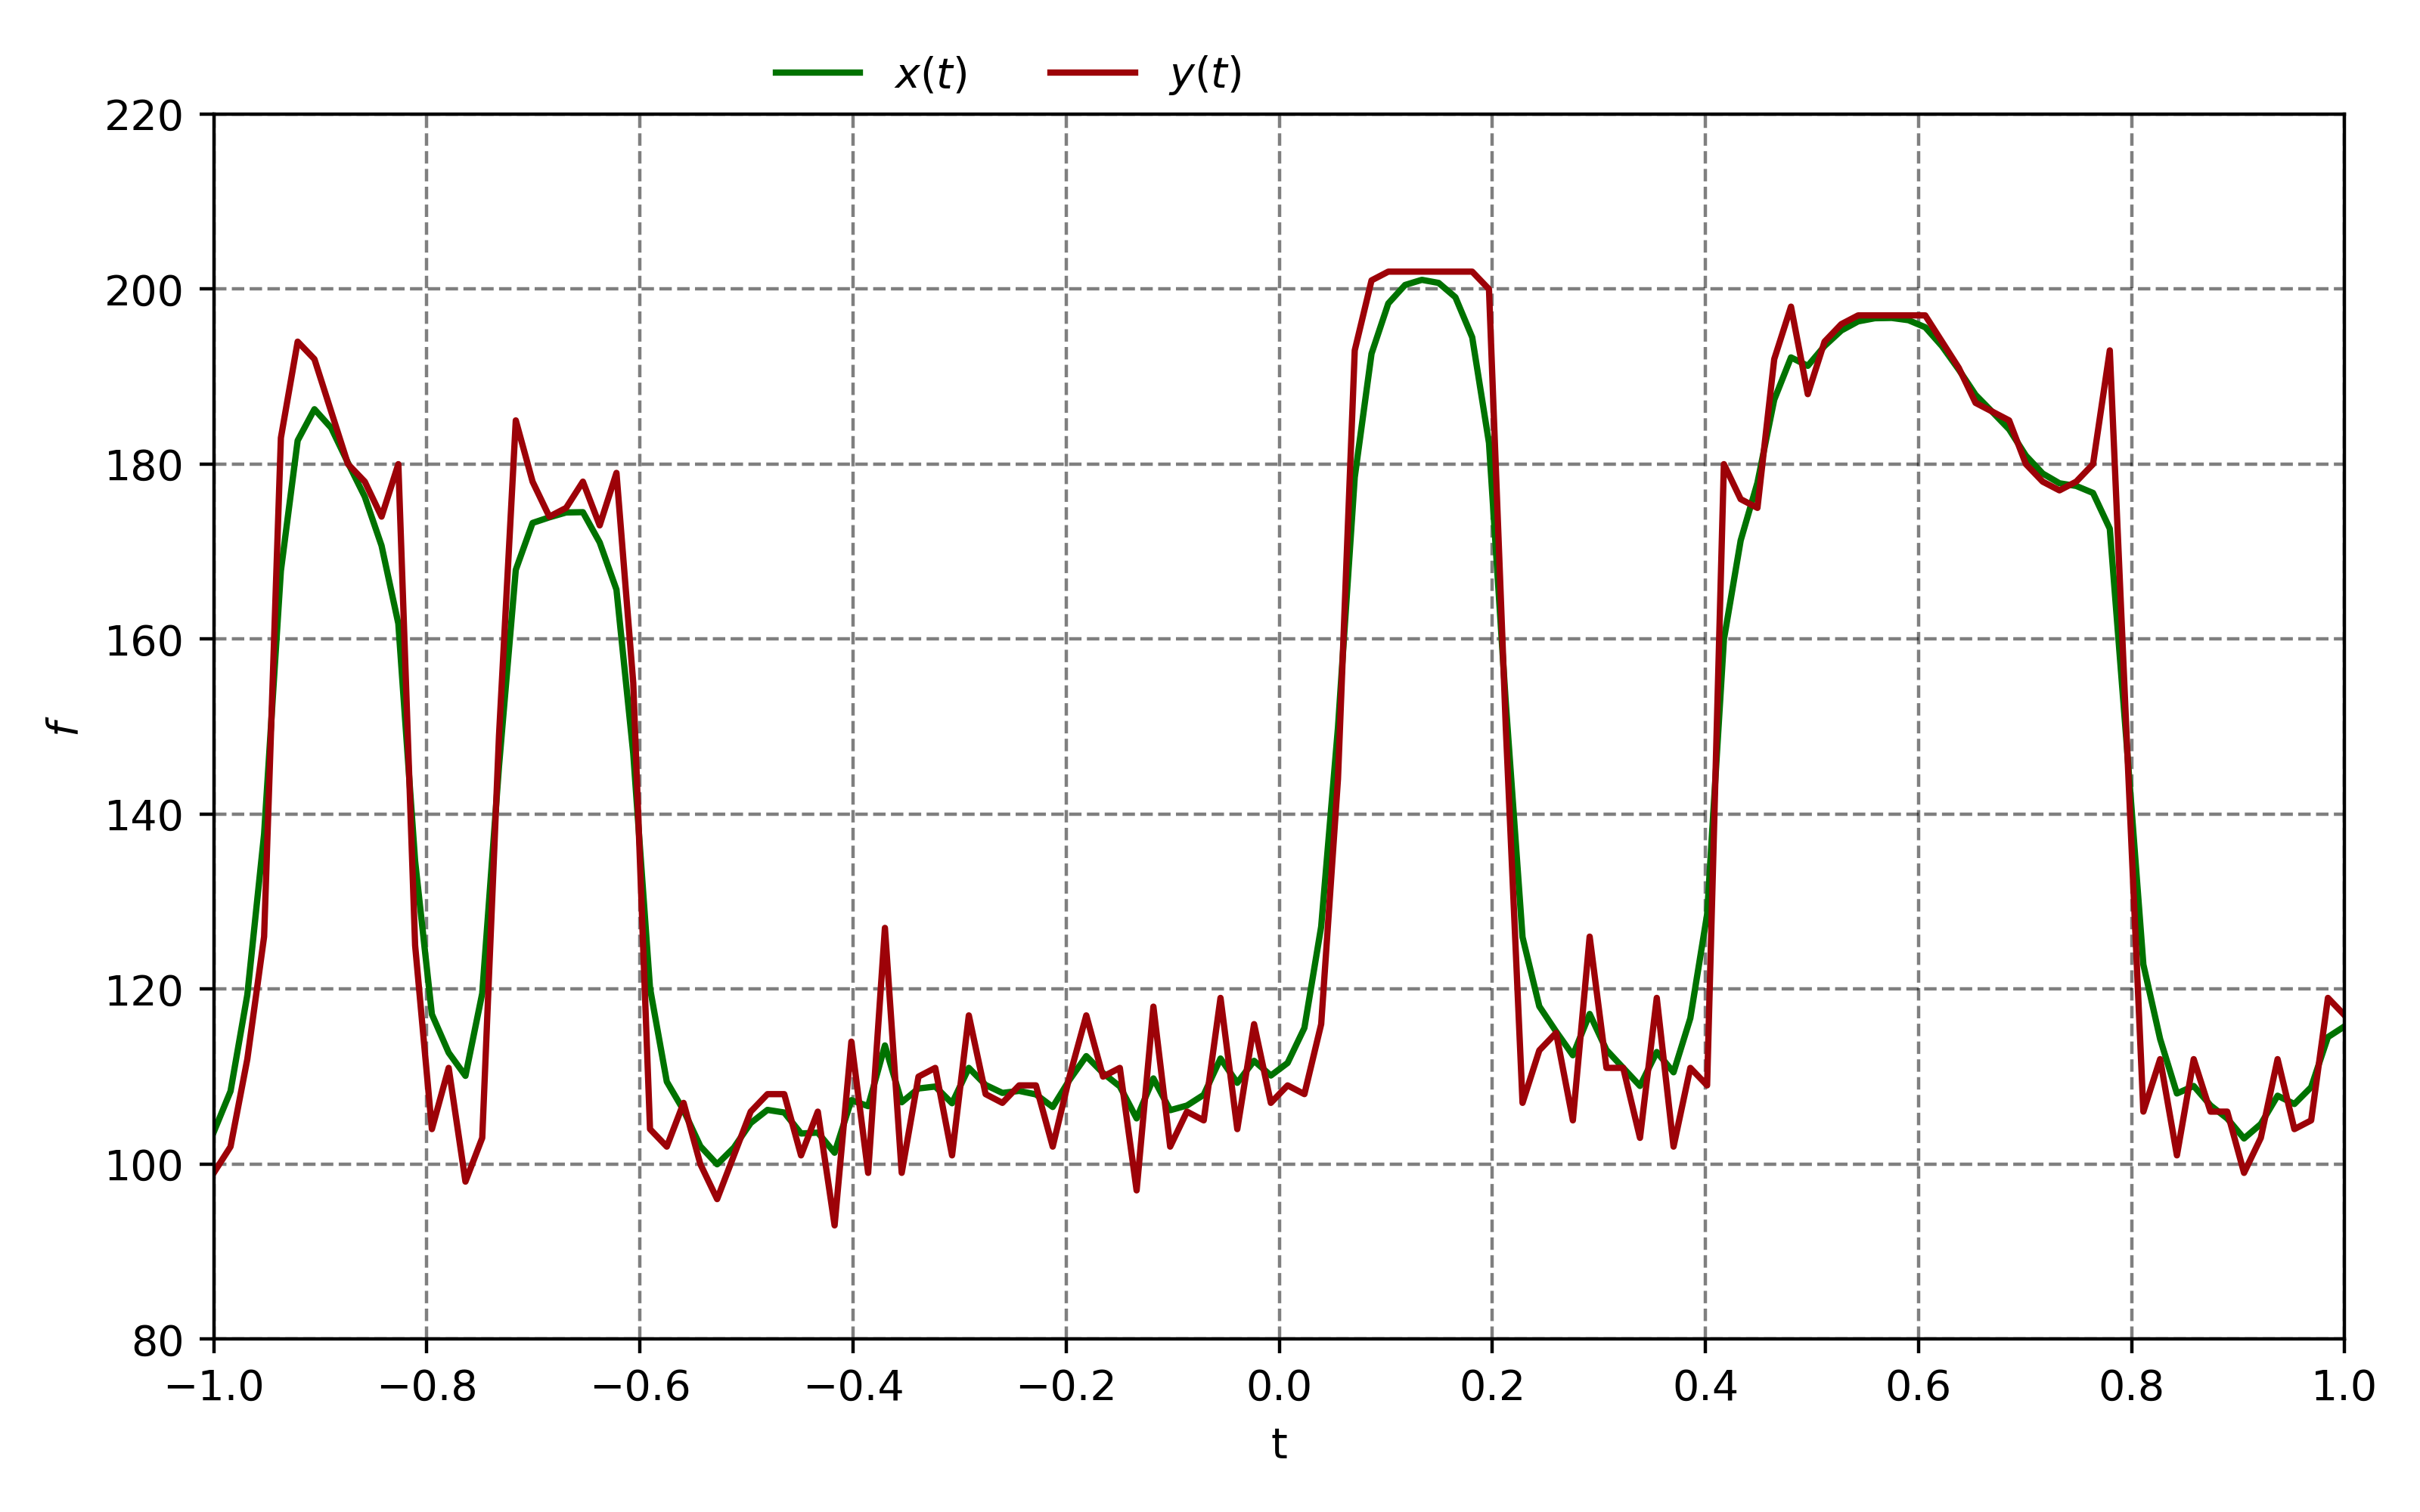
\includegraphics[width=17cm]{Graphics/Problema_3/lambda_1_test.png}
    \caption{Comparación de los valores de entrada del archivo \file{y.txt} ($y(t)$) con los valores obtenidos $(x(t))$ al realizar el suavizado usando el método del descenso de gradiente.}
    \label{fig:lambda_1_test}
\end{figure}

\paragraph{Vector aleatorio}

En la figura \ref{fig:lambda_1} se muestran los resultados de las funciones $x(t)$ y el vector aleatorio $y$ para el caso $\lambda=1$.

\begin{figure}[H]
    \centering
    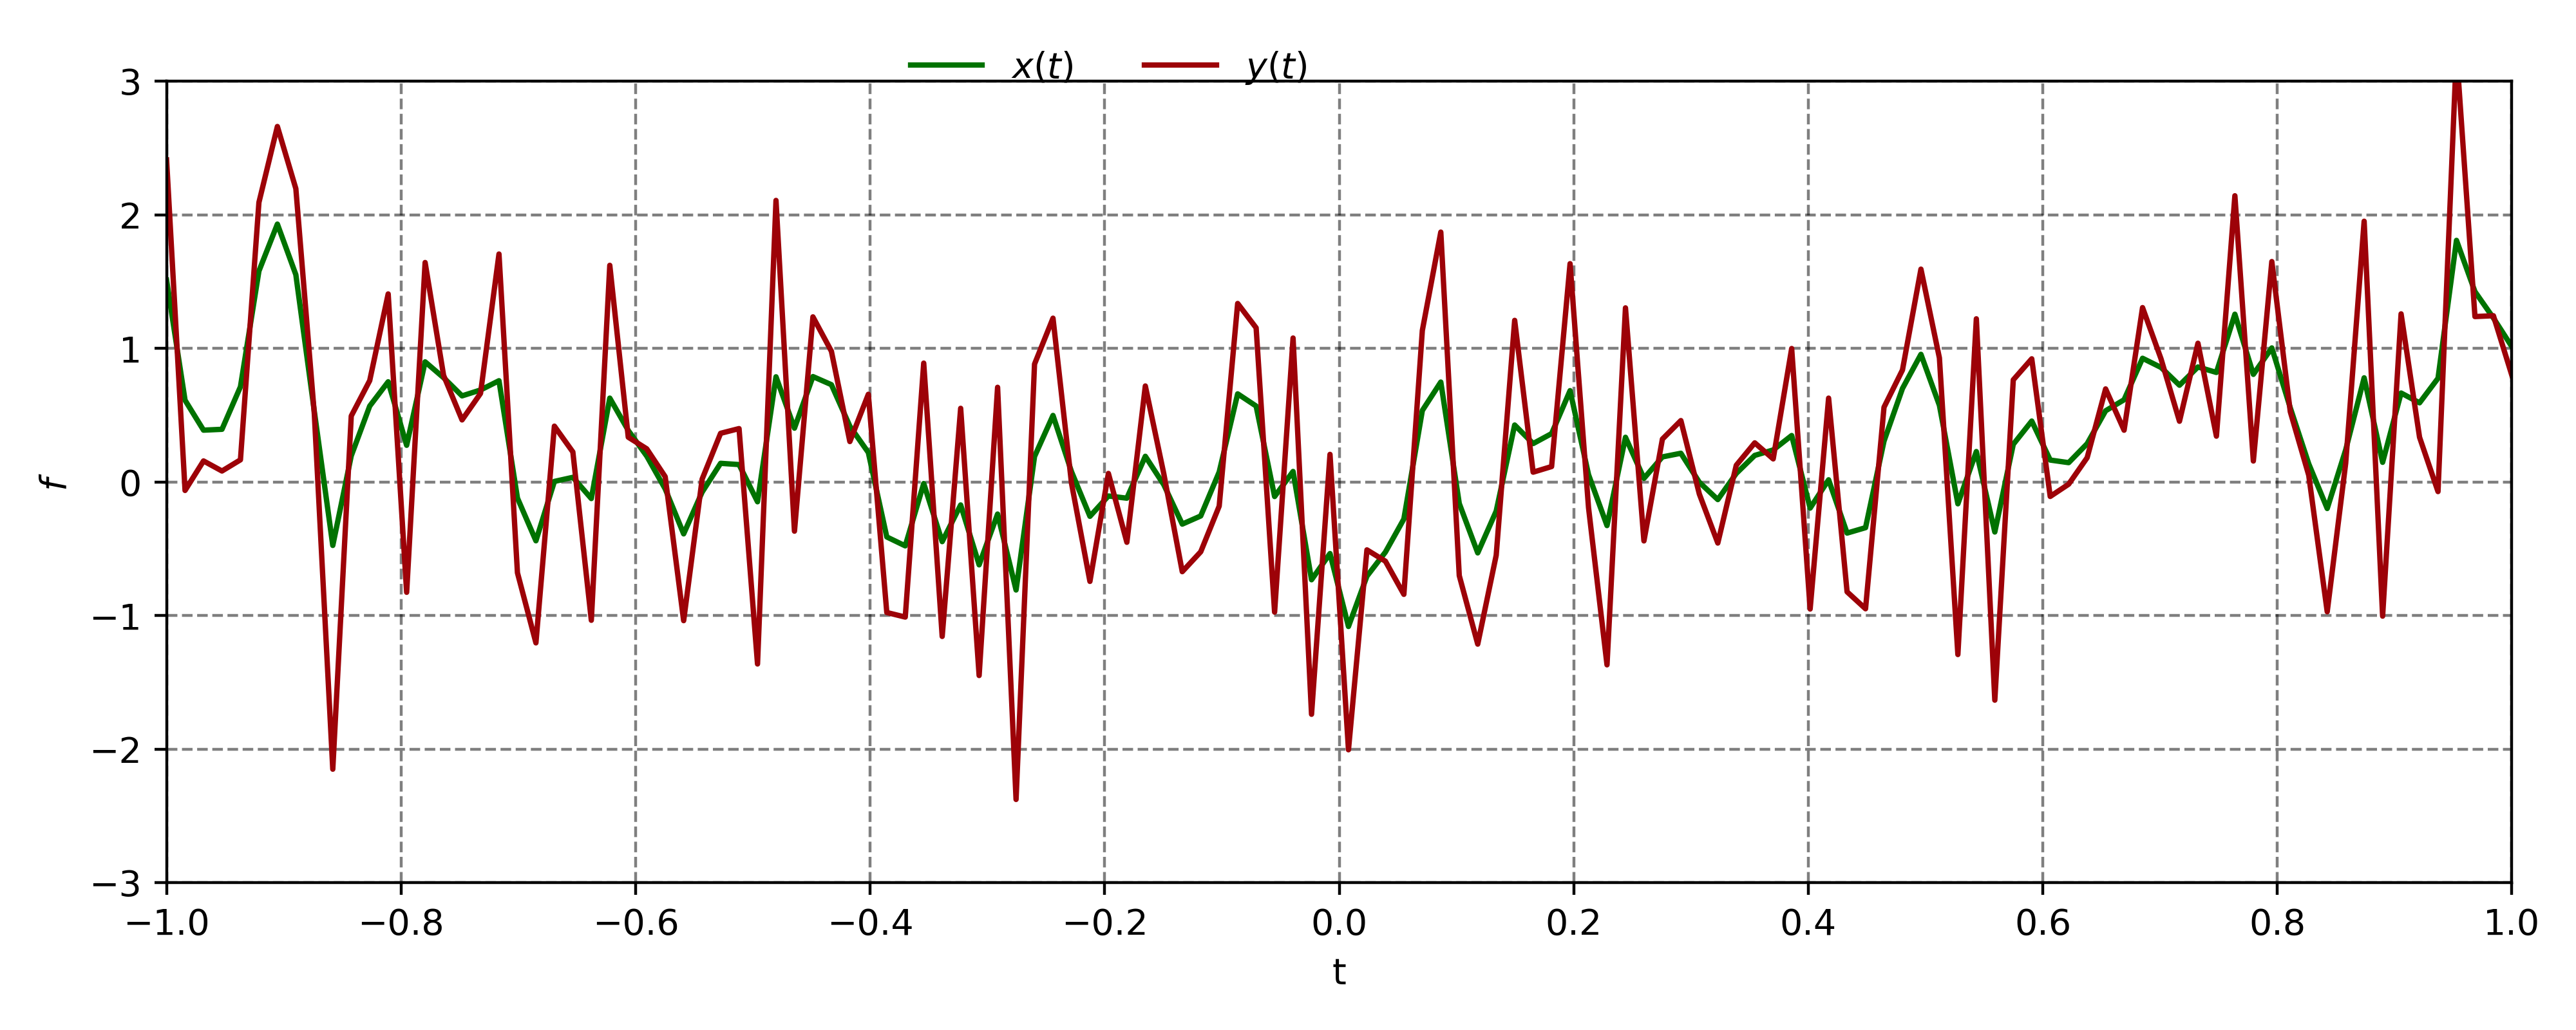
\includegraphics[width=17cm]{Graphics/Problema_3/lambda_1.png}
    \caption{Comparación del vector aleatorio ($y$) con los valores obtenidos $(x)$ al realizar el suavizado usando el método del descenso de gradiente.}
    \label{fig:lambda_1}
\end{figure}

\subsubsection{Segundo caso.}

\paragraph{Vector y predefinido}

En la figura \ref{fig:lambda_10_test} se muestran los resultados de las funciones $x(t)$ y el vector predefinido en el archivo \file{y.txt} para el caso $\lambda=10$.

\begin{figure}[H]
    \centering
    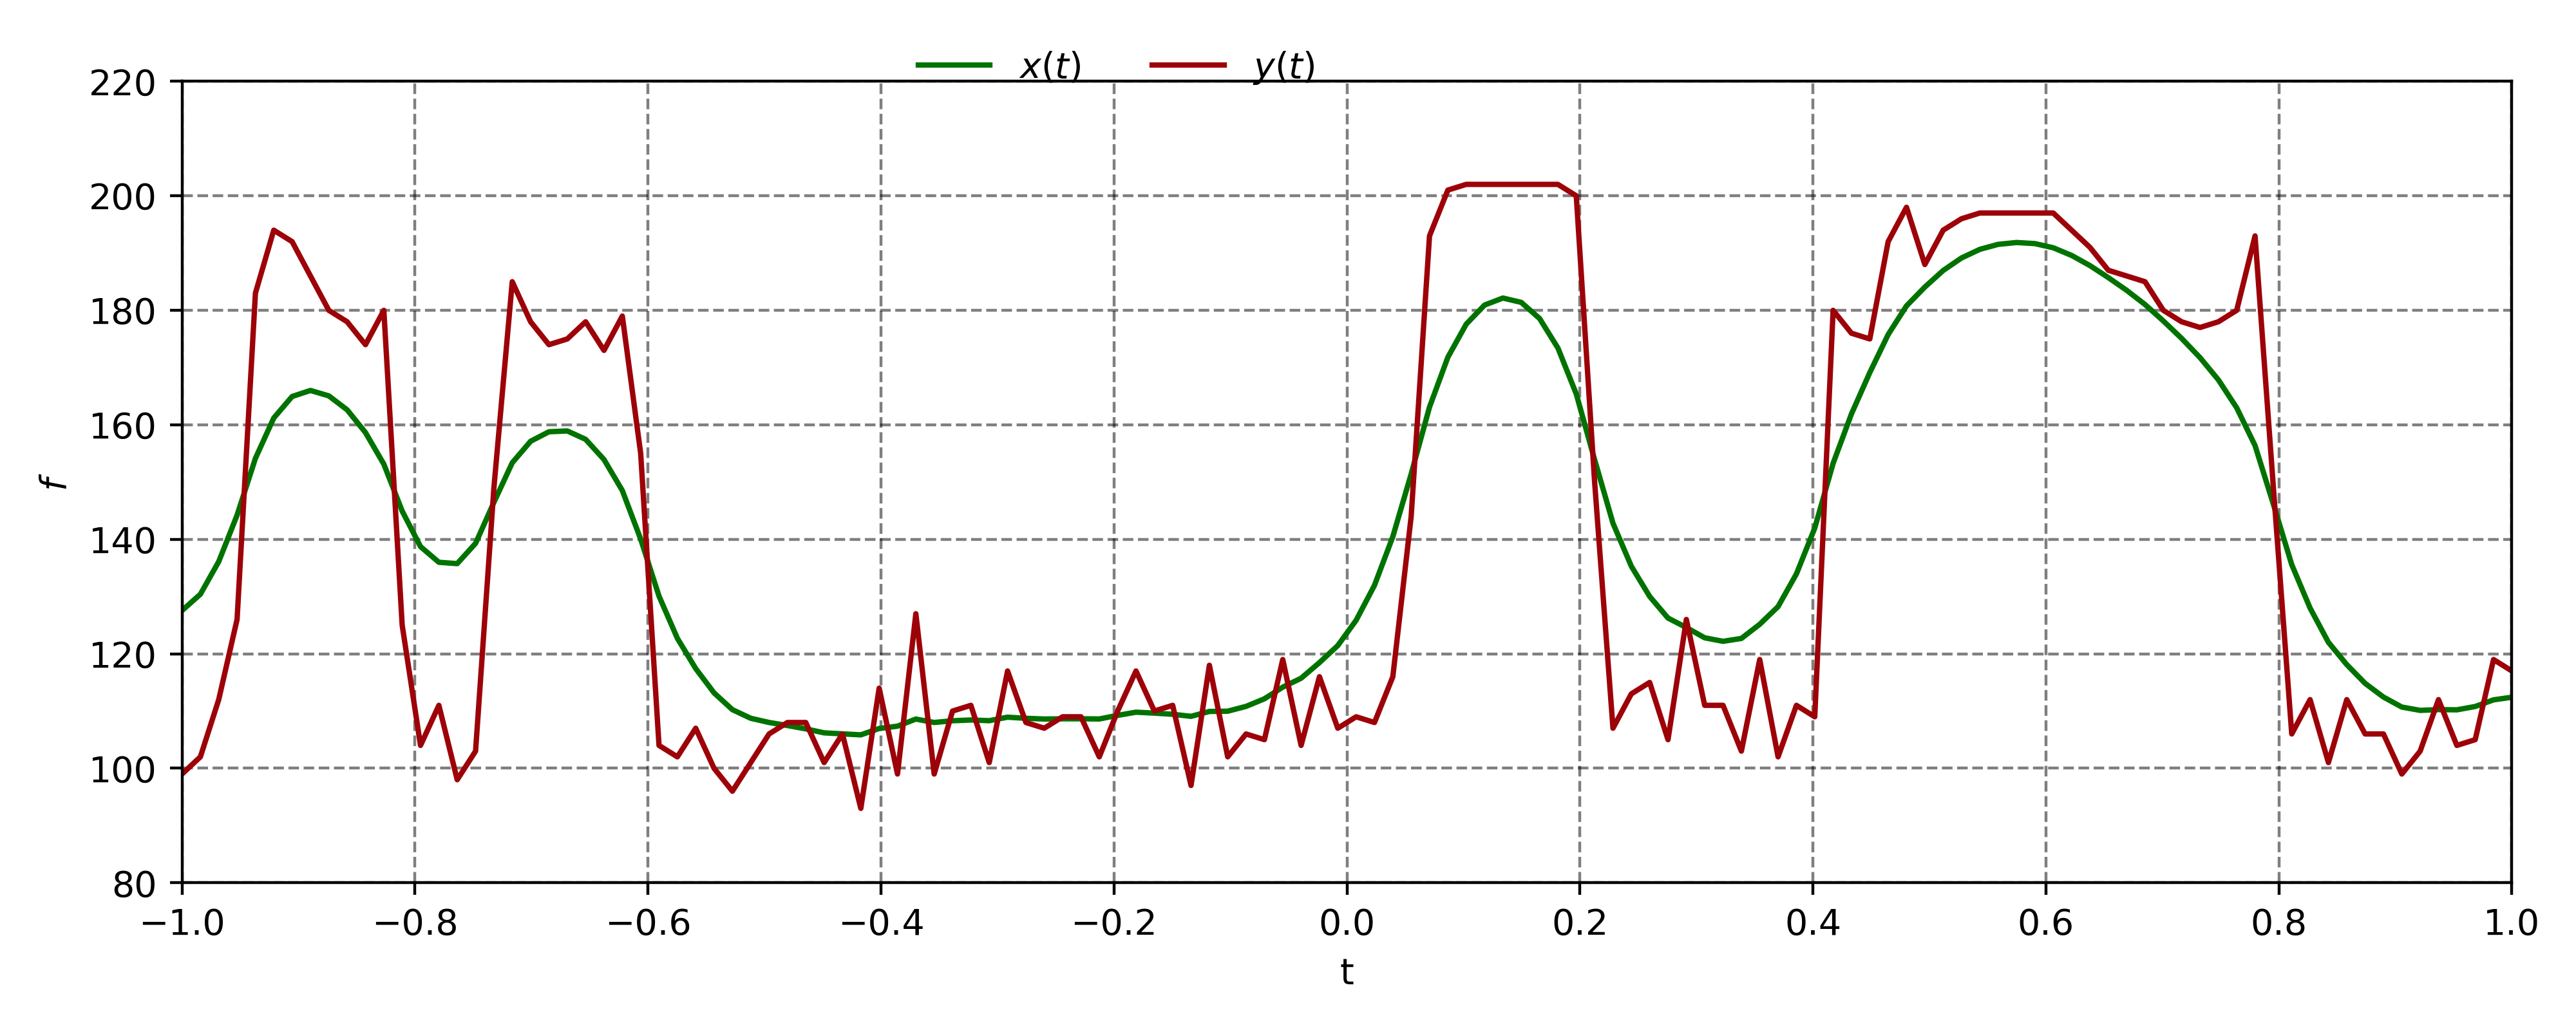
\includegraphics[width=17cm]{Graphics/Problema_3/lambda_10_test.png}
    \caption{Comparación de los valores de entrada del archivo \file{y.txt} ($y(t)$) con los valores obtenidos $(x(t))$ al realizar el suavizado usando el método del descenso de gradiente.}
    \label{fig:lambda_10_test}
\end{figure}

\paragraph{Vector aleatorio}

En la figura \ref{fig:lambda_10} se muestran los resultados de las funciones $x(t)$ y el vector aleatorio $y$ para el caso $\lambda=10$.

\begin{figure}[H]
    \centering
    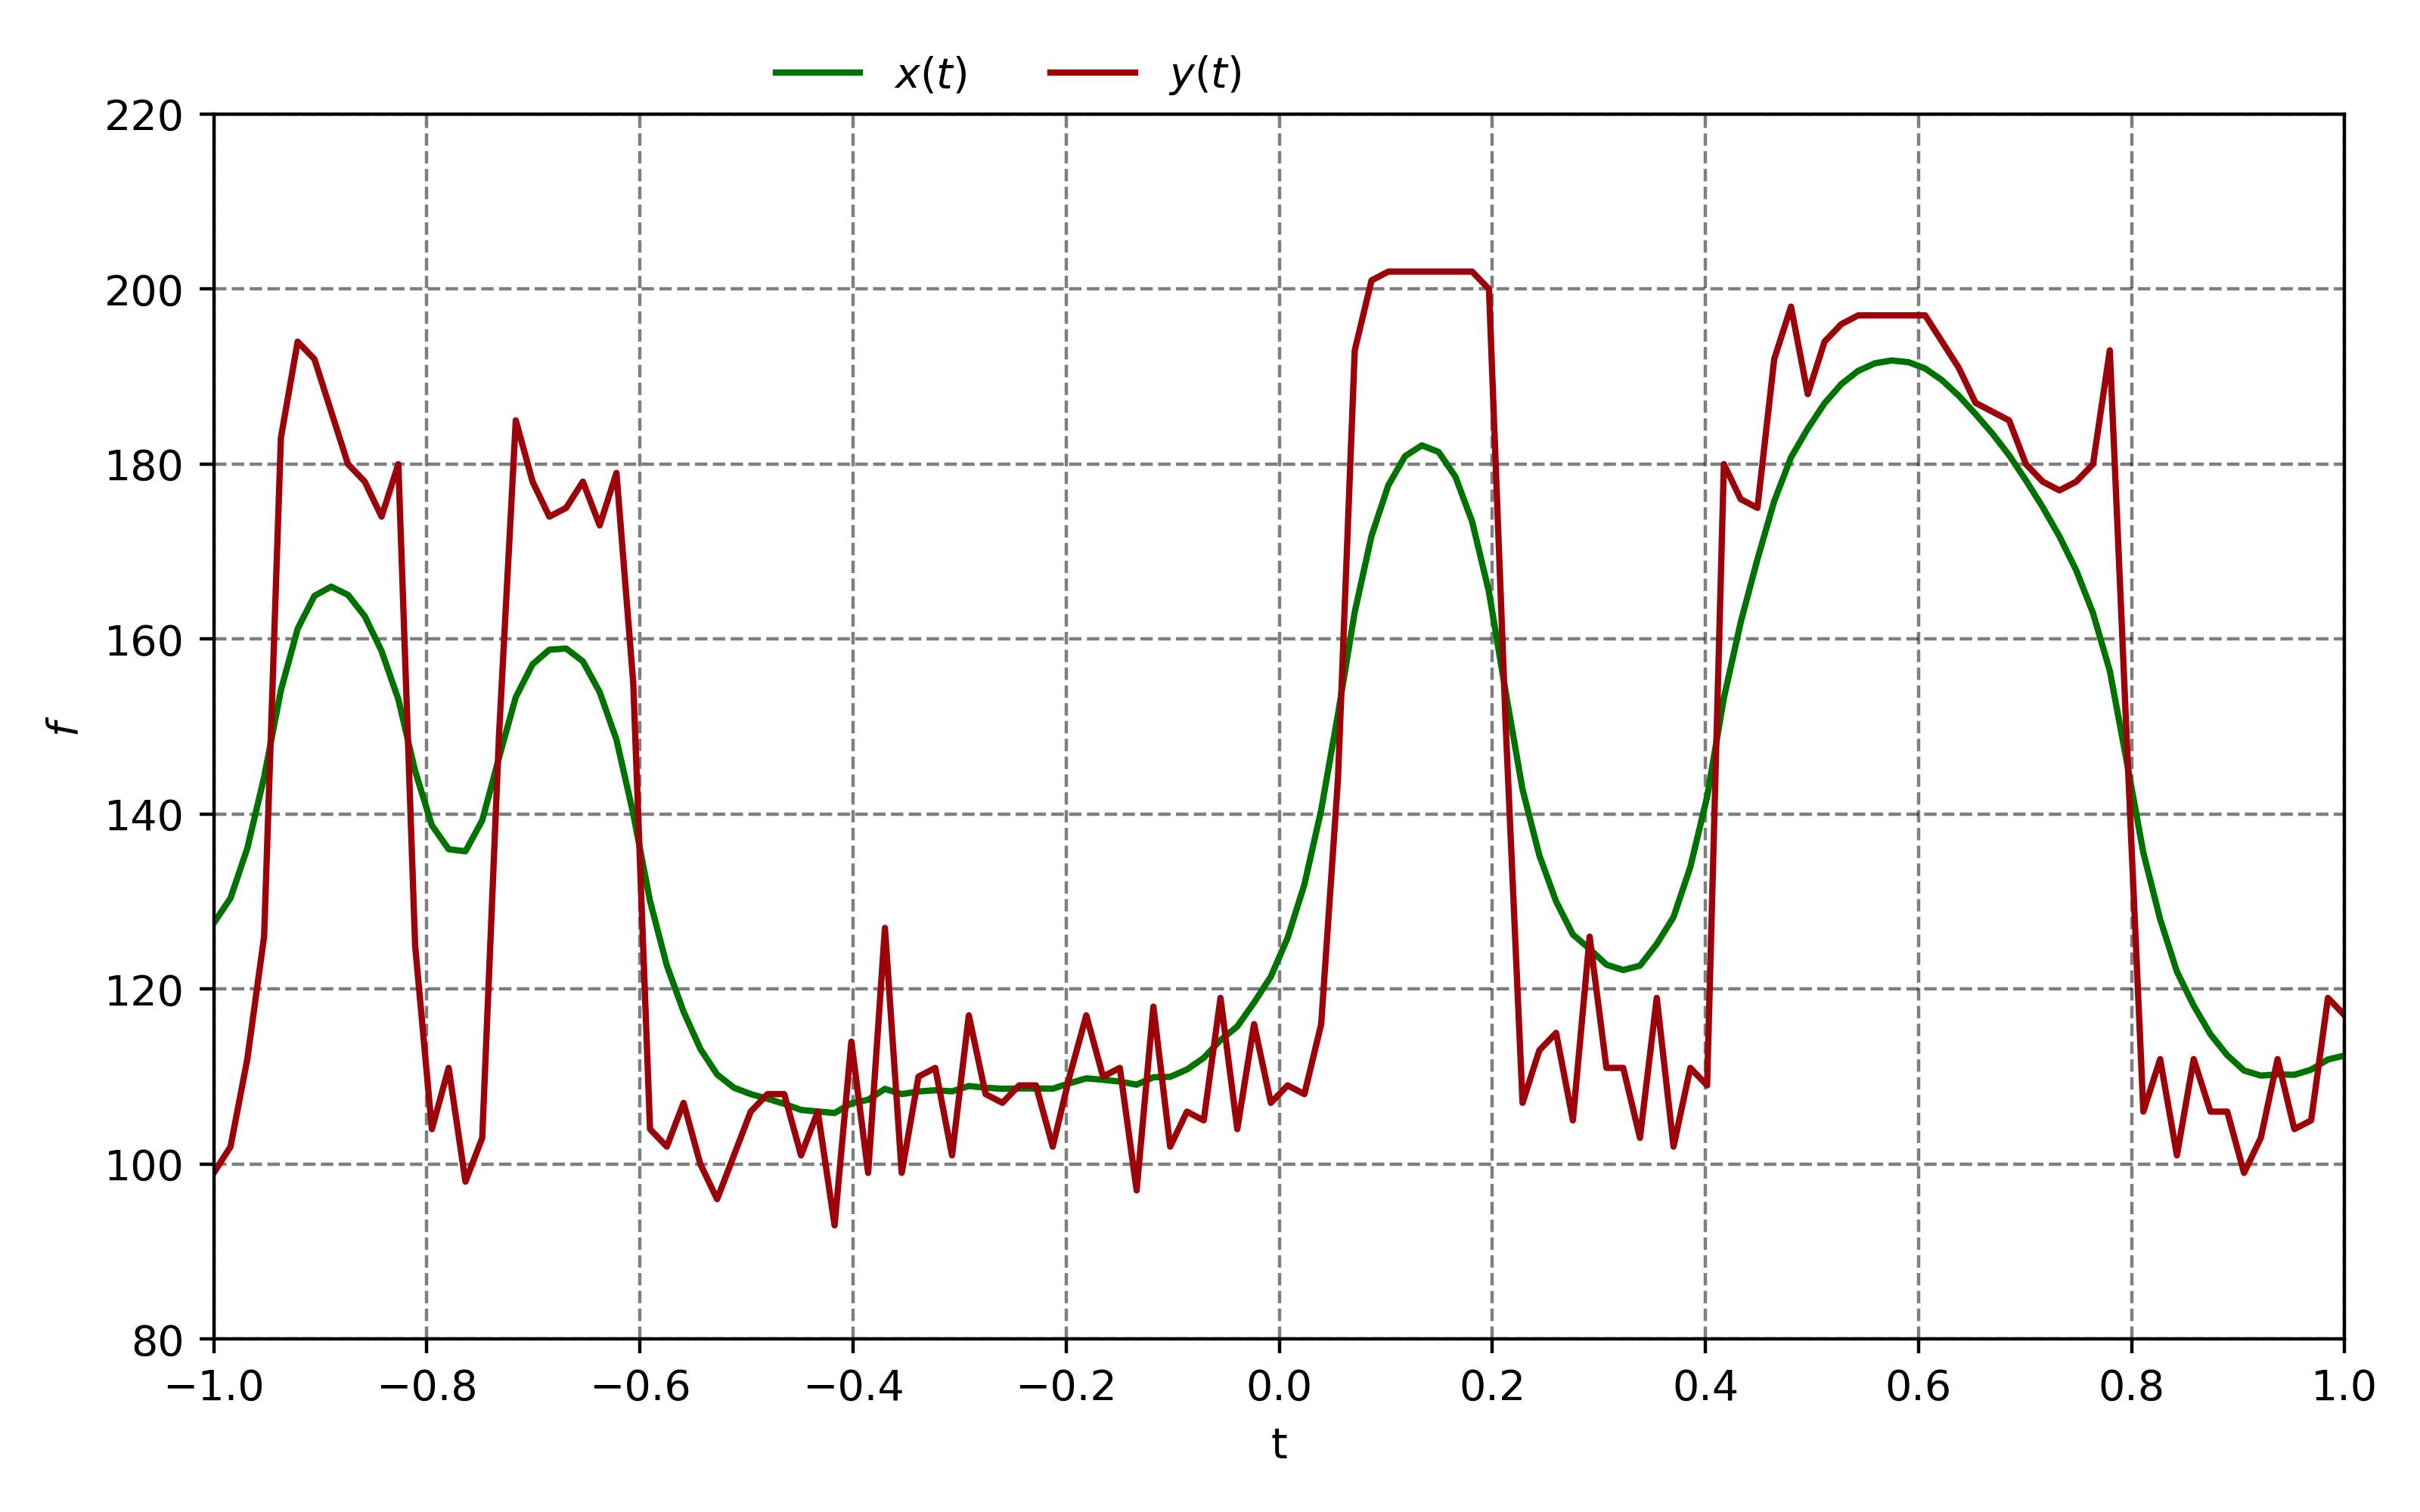
\includegraphics[width=17cm]{Graphics/Problema_3/lambda_10.png}
    \caption{Comparación del vector aleatorio ($y(t)$) con los valores obtenidos $(x(t))$ al realizar el suavizado usando el método del descenso de gradiente.}
    \label{fig:lambda_10}
\end{figure}

\subsubsection{Tercer caso.}

\paragraph{Vector predefinido}

En la figura \ref{fig:lambda_1000_test} se muestran los resultados de las funciones $x(t)$ y el vector predefinido en el archivo \file{y.txt} para el caso $\lambda=1000$.

\begin{figure}[H]
    \centering
    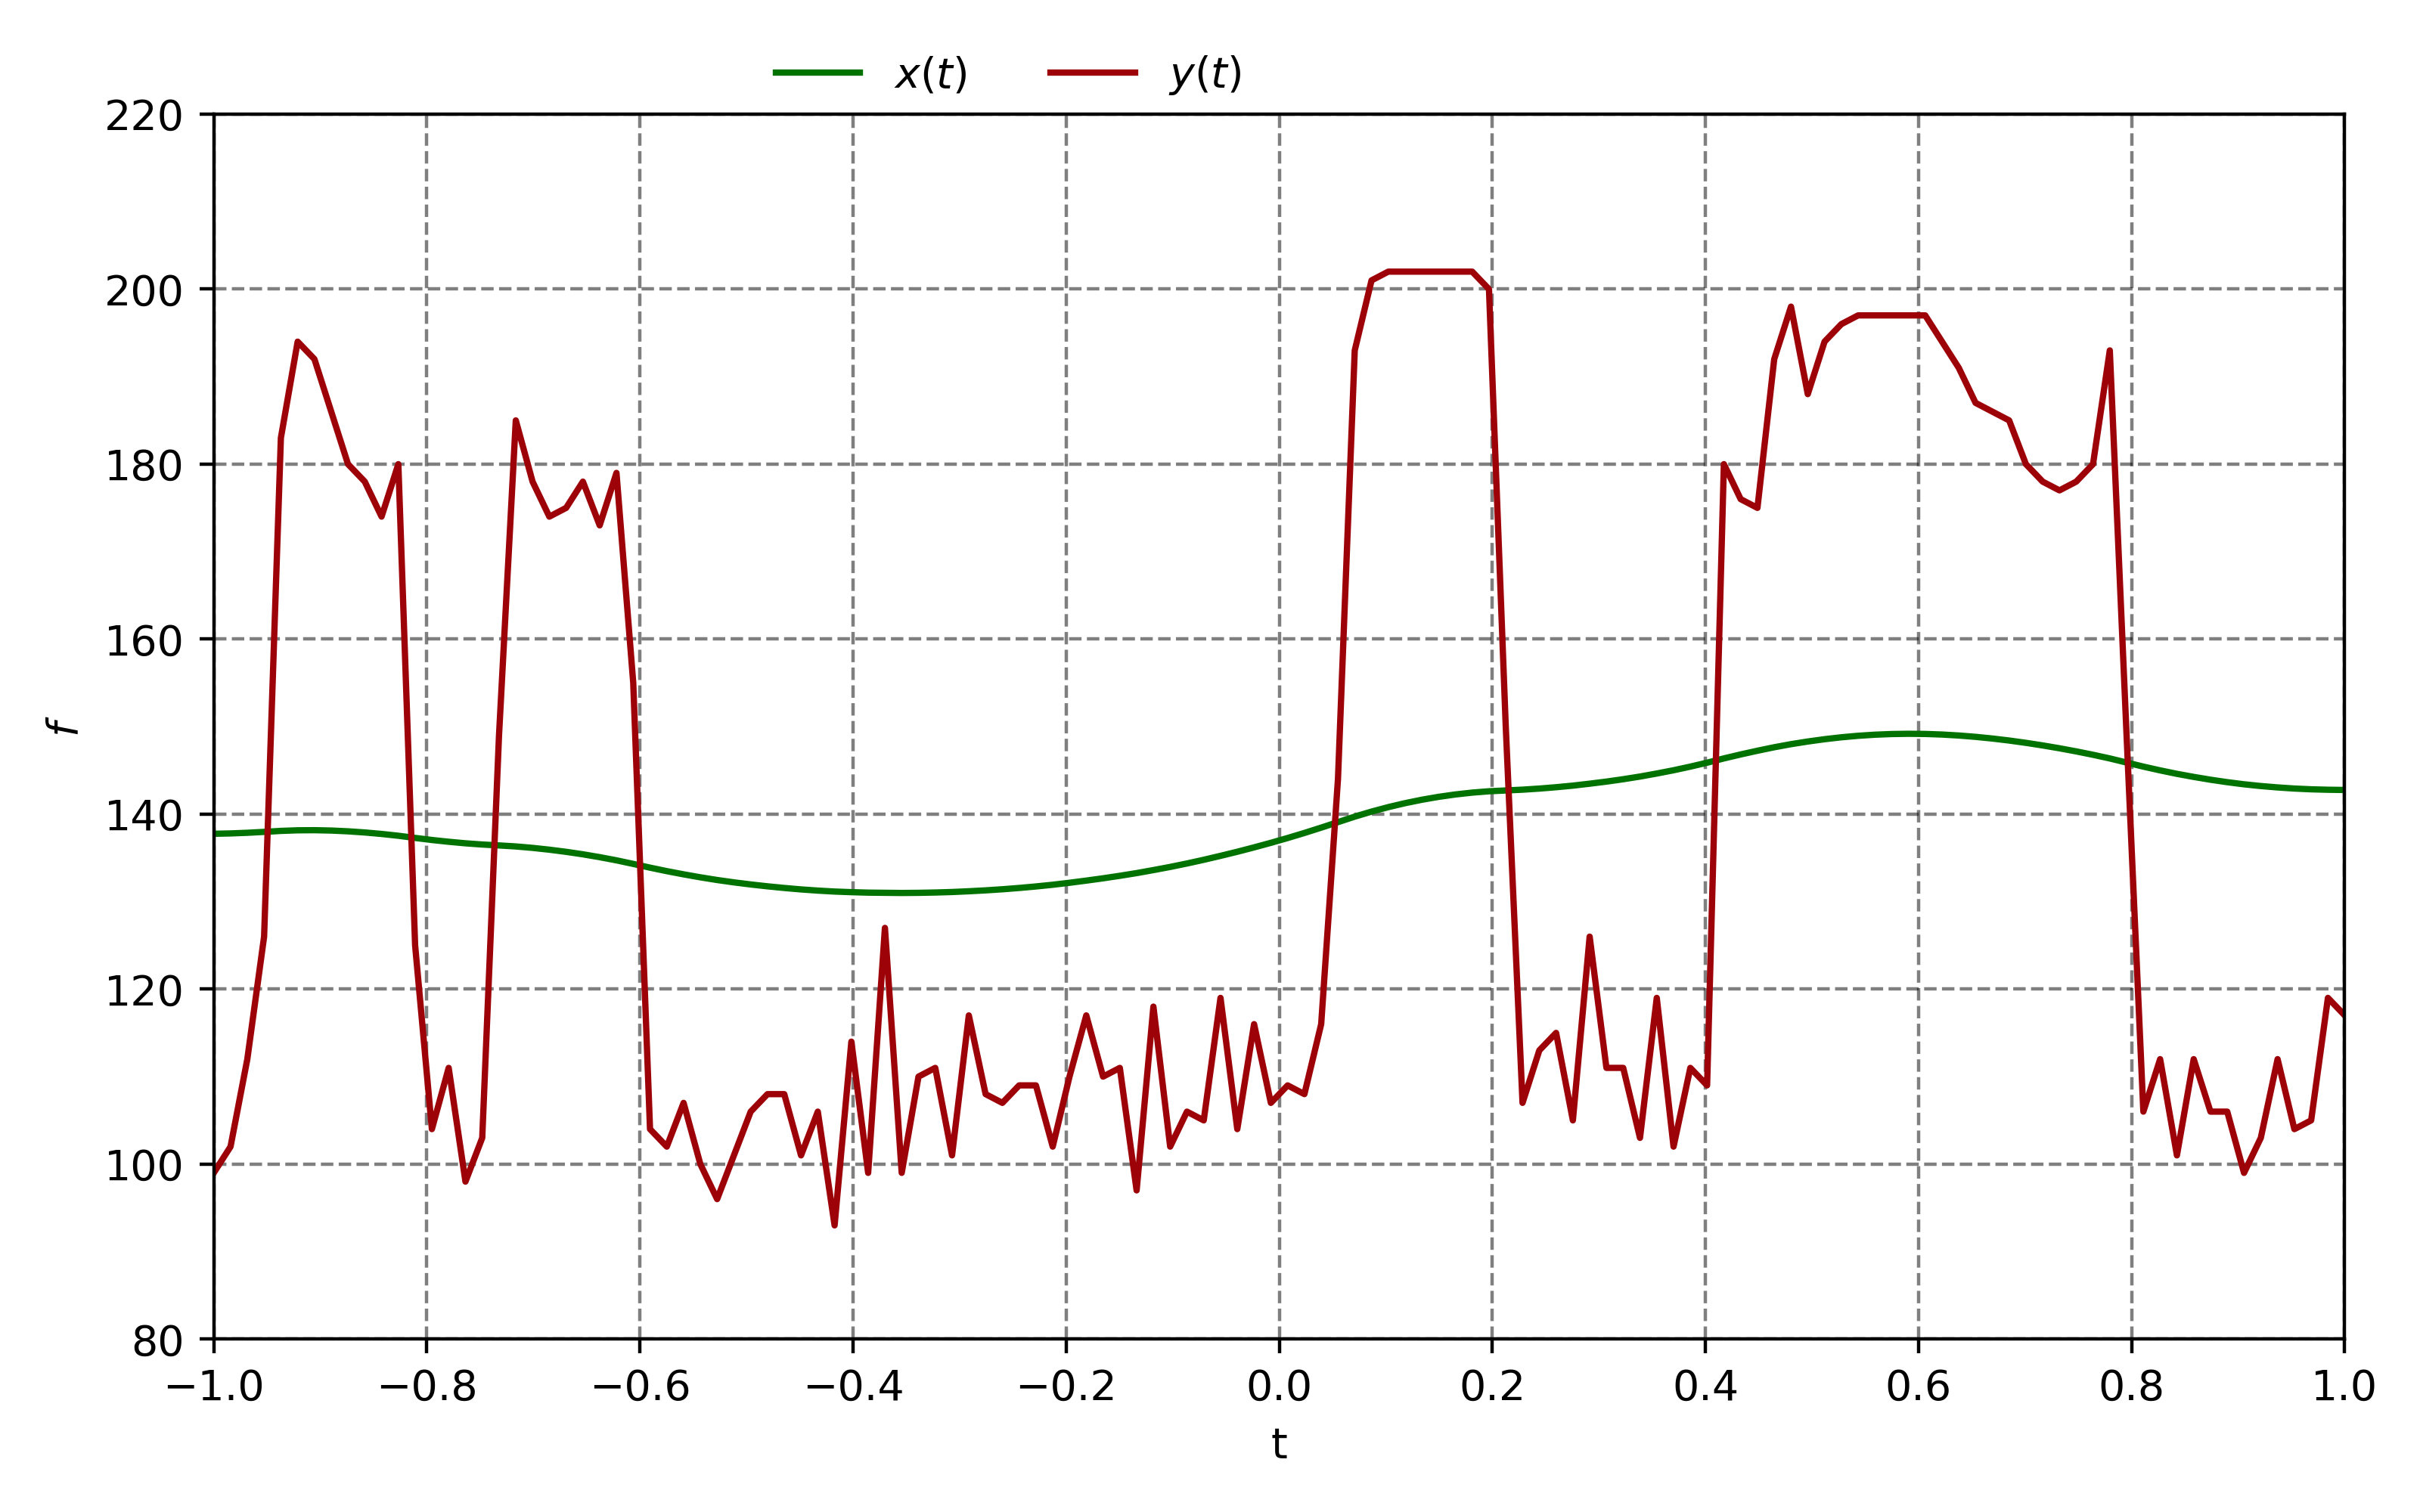
\includegraphics[width=17cm]{Graphics/Problema_3/lambda_1000_test.png}
    \caption{Comparación de los valores de entrada del archivo \file{y.txt} ($y(t)$) con los valores obtenidos $(x(t))$ al realizar el suavizado usando el método del descenso de gradiente.}
    \label{fig:lambda_1000_test}
\end{figure}

\paragraph{Vector y aleatorio}

En la figura \ref{fig:lambda_1000} se muestran los resultados de las funciones $x(t)$ y el vector aleatorio $y$ para el caso $\lambda=1000$.

\begin{figure}[H]
    \centering
    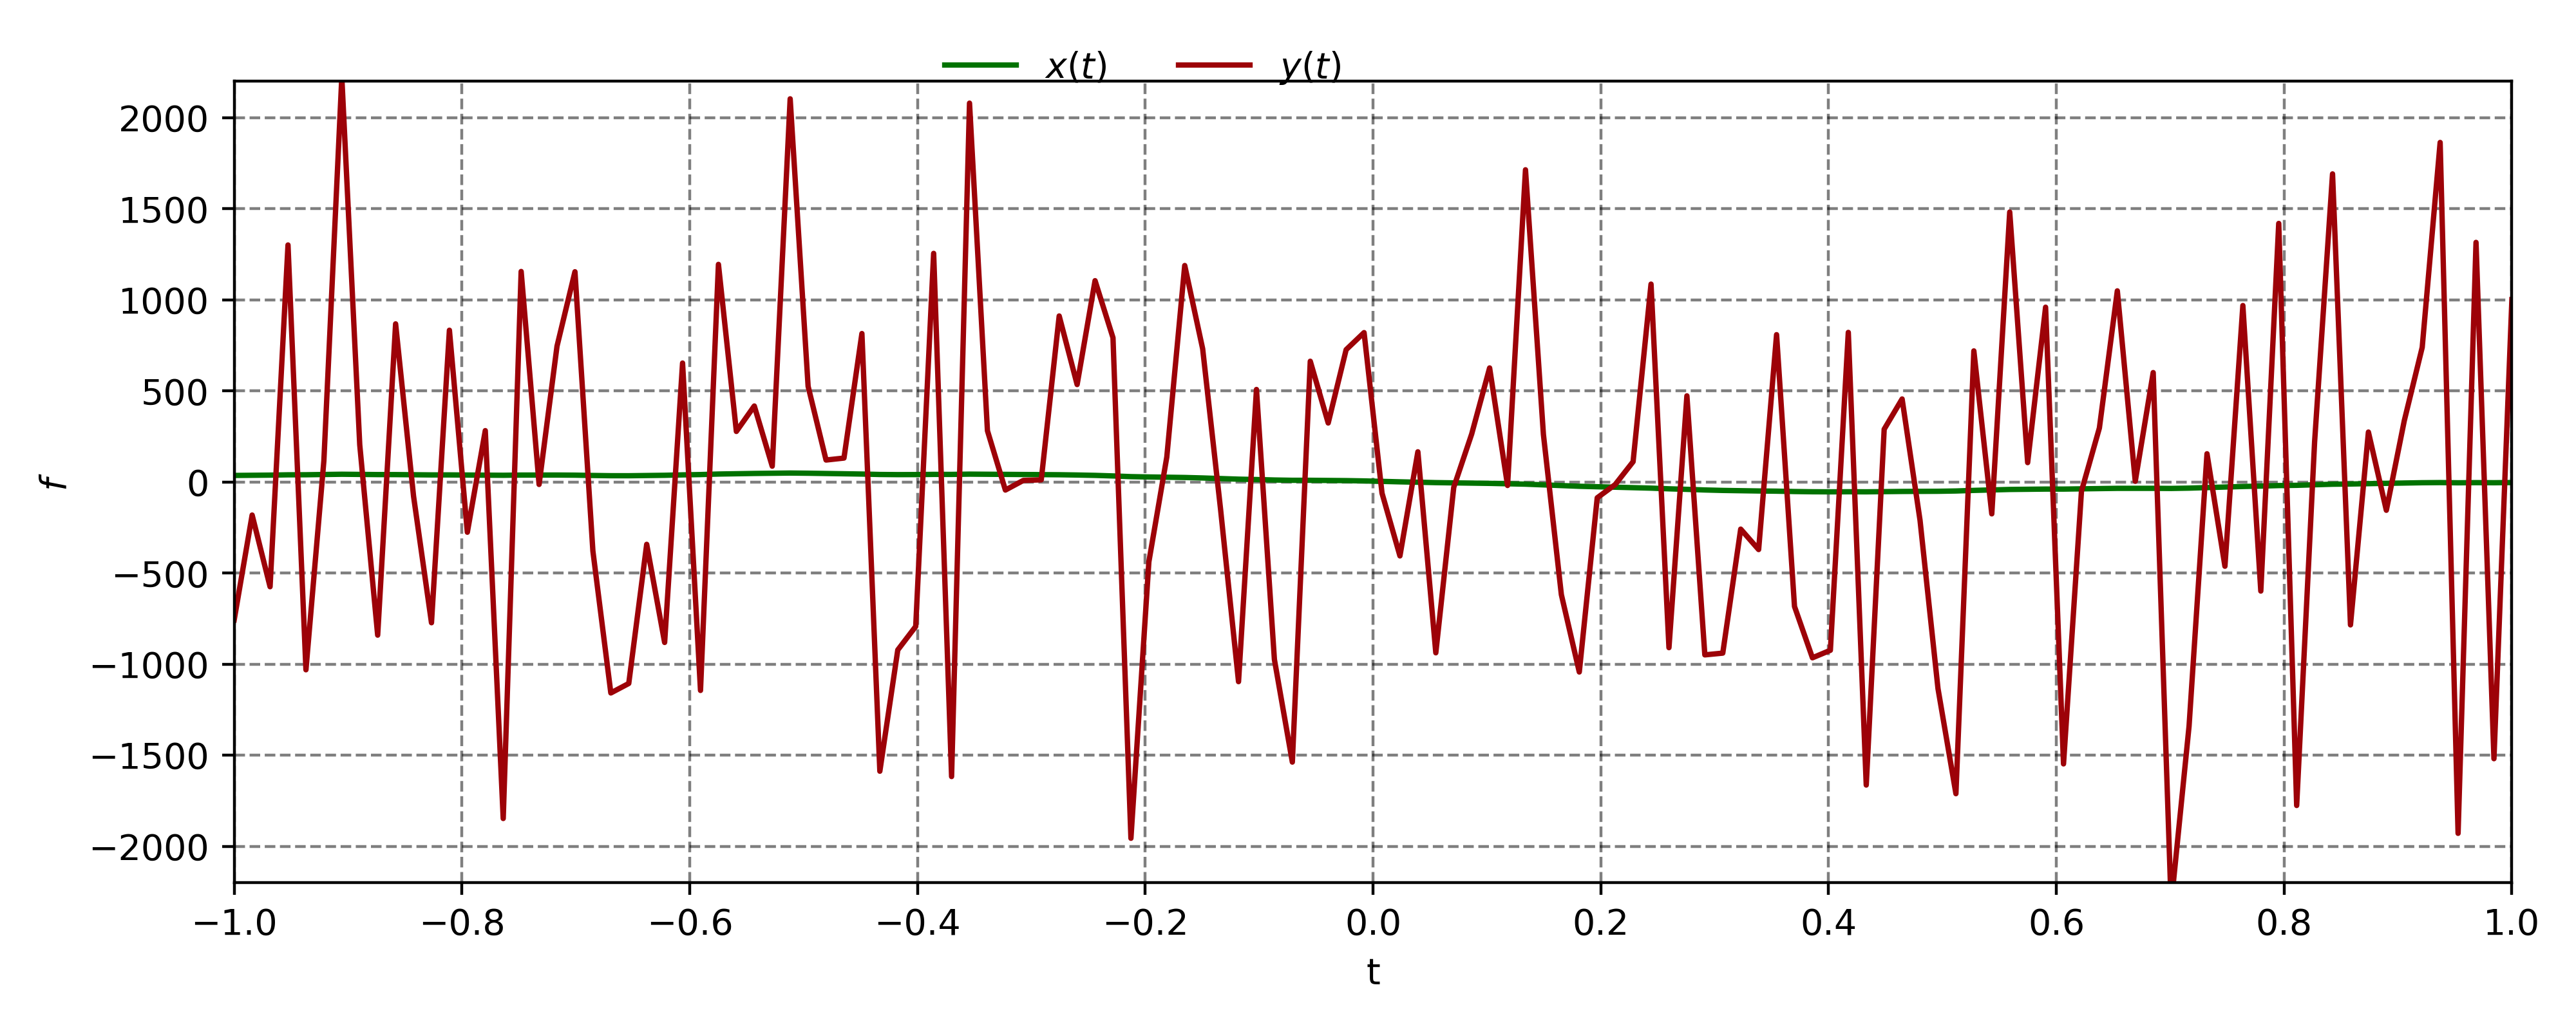
\includegraphics[width=17cm]{Graphics/Problema_3/lambda_1000.png}
    \caption{Comparación del vector aleatorio ($y(t)$) con los valores obtenidos $(x(t))$ al realizar el suavizado usando el método del descenso de gradiente.}
    \label{fig:lambda_1000}
\end{figure}